% ============================================================
% Chapter 1: Introduction — 本文（Phase 2, 2026-09-07）
% 骨子版（Phase 1, P1-P8）は git 履歴を参照。段落構成は骨子どおり:
%   P1 問題 / P2 AutoPMoB（図 1）/ P3 本研究の課題と「集合」の必然性（CSTR）/ P4 手法 /
%   P5 データと分割 / P6 結果 / P7 貢献 / P8 章構成
% 数値の一次ソースは各段落の % source: コメントに記載（2026-09-07 に JSON と照合）。
% 図 1 は generate_figures_thesis.py overview() で生成（figures/fig_autopmob_overview.pdf）。
% 設計書: docs/superpowers/specs/2026-09-07-w2-introduction-design.md
% ============================================================

Physical models --- systems of equations that describe how the material, energy, and momentum
of a process change --- underpin the process industry. Process design sizes equipment on them,
process control tunes controllers on them, and a digital twin keeps such a model in step with the
running plant\cite{DigitalTwin}. Purpose-built tools such as MATLAB/Simulink\cite{simulink} and
Aspen Plus\cite{aspen} let an engineer assemble a model quickly, but only for the unit operations
and phenomena that their libraries already cover. For a process outside those libraries, the
engineer surveys a large body of papers, textbooks, and handbooks, collects the equations
scattered across them, and refines a prototype model by trial and error. Modeling a new process
is therefore slow, and it depends on the few experts who can read the literature of the field.

To free engineers from this work, our group aims to develop an automated physical model builder,
AutoPMoB\cite{AutoPMoBCSTR,AutoPMoBProto}. Fig.~\ref{fig:overview}(a) shows its pipeline:
AutoPMoB collects documents about a target process, extracts equations, variables, and
experimental data from them, judges which extracted items are equivalent across documents, and
reorganizes the equivalent items into the desired model. Our group has developed its component
technologies step by step: an annotation tool and an extraction algorithm collect variable symbols
from engineering documents\cite{VARAT}, a language model pre-trained on a chemical-engineering
corpus judges whether two variable definitions refer to the same quantity\cite{ProcessBERT}, and
a computer-algebra algorithm judges whether two equation systems are
equivalent\cite{DAEEquiv}.

\begin{figure}[htb]\centering
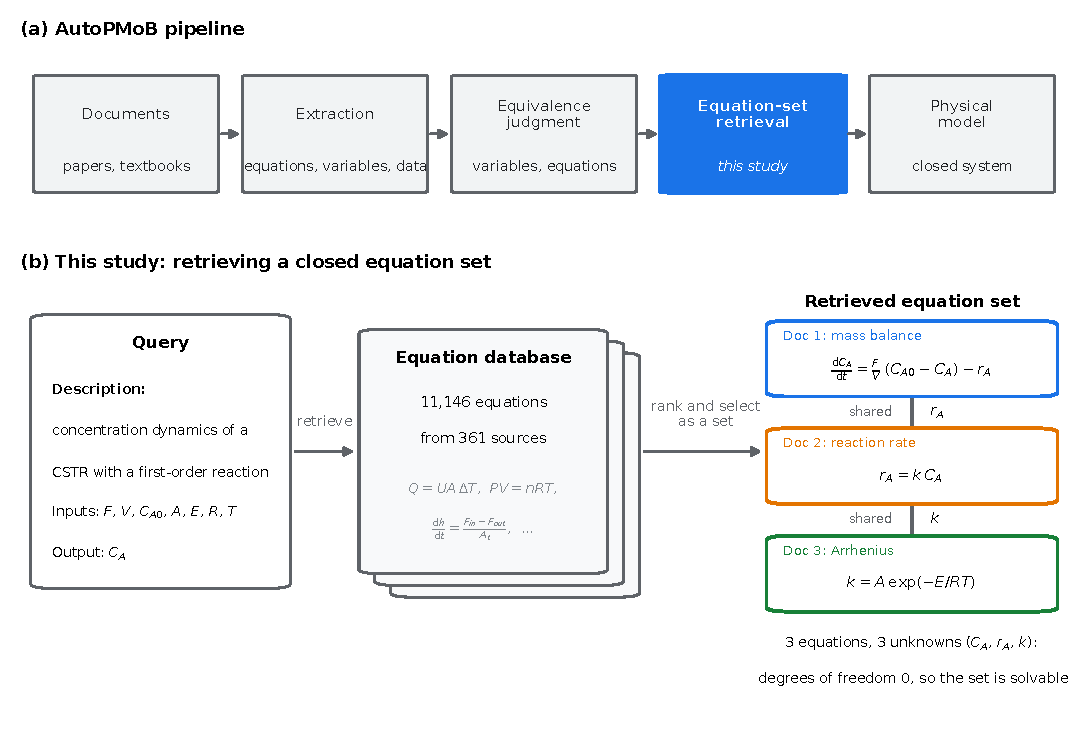
\includegraphics[width=0.98\linewidth]{figures/fig_autopmob_overview.pdf}
\caption{The automated physical model builder (AutoPMoB) and the position of this study. (a)
AutoPMoB collects documents about a target process, extracts equations, variables, and data,
judges their equivalence across documents, and reorganizes them into the desired model; this
study addresses the highlighted stage. (b) The task of this study: a query gives a description of
the desired model with its input and output variables, and the method retrieves, from a database
of 11,146 equations drawn from 361 sources, the set of equations that composes the model. The
three retrieved equations come from different documents and are linked by the variables they
share ($r_A$ and $k$); with three equations and three unknowns ($C_A$, $r_A$, and $k$) the set
has zero degrees of freedom, so a simulator can solve it.}
\label{fig:overview}
\end{figure}

This study addresses the reorganization step, the highlighted stage of
Fig.~\ref{fig:overview}(a): given a description of the desired model together with its input and
output variables, retrieve the set of equations that composes the model from an equation database
built from many documents (Fig.~\ref{fig:overview}(b)). The step is a retrieval problem with an
unusual answer. A physical model is not a list of independent equations but a system of equations
that share variables and must be solved simultaneously, and the system can be solved only when it
has as many equations as unknown variables --- when its degrees of freedom are zero --- so that,
once the inputs are given, every output is determined. The concentration dynamics of a continuous
stirred-tank reactor (CSTR), for example, need three coupled equations: the mass-balance ordinary
differential equation (ODE) for the concentration, the reaction-rate equation $r_A = k C_A$, and
the Arrhenius equation $k = A\exp(-E/RT)$ for the rate constant. The ODE alone leaves the rate
$r_A$ undetermined, the rate equation alone leaves the rate constant $k$ undetermined, and only
the three together close the system. A method that scores each equation by its similarity to the
description cannot see these dependencies: each of the three equations looks only moderately
relevant on its own, an equation from an unrelated document may look more relevant than any of
them, and no similarity score tells whether a set of equations closes. Retrieval must therefore
evaluate candidate equations as a set, not one by one.

We propose a two-stage retrieval method whose second stage evaluates each candidate against the
equations already selected. The first stage ranks the whole database by a mixture of text
similarity and variable overlap and keeps the top candidates. The second stage reranks the
candidates with a multilayer perceptron (MLP) that reads ten features per candidate: seven
features of the query--equation pair, such as the text similarity and the fraction of the query
variables the equation contains, and three set-aware features that compare the candidate with a
reference set --- the top-ranked candidates or, in the sequential variants, the equations already
selected. The set-aware features ask whether the candidate supplies query variables the reference
set still lacks (complementarity), whether it shares variables with the set (coherence), and
whether it comes from the same field (domain agreement). We further introduce a learned greedy
selection that builds the set one equation at a time and trains with teacher forcing so that
training and inference see the same sequential context, and a self-terminating criterion
that halts retrieval when the selected set closes as a system (DoF-stop, named after the degrees
of freedom it monitors). The method thus returns
a ranked, solvable equation set without being told how many equations the answer has.

To evaluate the method under realistic difficulty, we construct a large equation database and
test cases whose answers are solvable, and we split them so that no document leaks between
training and testing. The database holds 11,146 equations from 361 sources, extracted from the
documents by a large language model (LLM) and normalized in notation. The 2,838 cases fall into
three families by how their answer sets were formed --- as published in one document, assembled
across documents, or synthesized --- plus augmented copies used only for training; the 1,000
synthesized cases grow by a rule that adds variable-sharing equations until the system closes, so
their answers are solvable by construction. We assign every source wholly to training,
validation, or testing, and we stratify the assignment so that four difficulty-related
distributions match between training and testing. All experiments repeat over 10 random splits
and report the mean and the spread.
% source: unified_equations.json（11,146 式・361 source）; training_cases.json（original 92 /
%         multisource_* 731 / dae_* 1,000 / 拡張 1,015 = 2,838）; 第 4 章 §4.1-4.4

Experiments show that the proposed method outperforms lexical and dense retrieval baselines and
direct generation by an LLM, and the analyses explain why. Recall@K --- the fraction of the
ground-truth equations found within the top $K$ of the ranking, where $K$ is the size of the
ground truth --- rises from 0.521 to 0.743 in the mixed setting and from 0.466 to 0.689 in the
hardest, synthesized-only setting, a gain of $+0.22$ in both on all 10 splits (Wilcoxon
signed-rank test, $p = 0.00195$).
% source: experiments/strat_A.json / strat_B.json results.*.Recall@K_correct（0.5206→0.7429,
%         0.4661→0.6890）; significance_stats.json（p_wilcoxon 0.00195）
Stronger text scorers do not close the gap: BM25 and a dense sentence encoder (E5), each mixed
with the variable-overlap term at its best weight, reach at most 0.602 and 0.555 in the two
settings, and an LLM that writes the equations directly reaches 0.23--0.30 even when a separate
model judges mathematical equivalence.
% source: experiments/external_baselines_stats.json best_per_scorer（A: bm25 0.6008 / e5io 0.6020;
%         B: bm25 0.5548 / e5io 0.5439）; llm_set_A/B/full_equiv_results.json（0.2545 / 0.2258 /
%         0.3003）
The analyses locate the cause of the gain in the structure of the answer rather than in its
topic: the set-aware features that read shared variables --- complementarity and coherence ---
carry the set-aware gain, domain agreement adds nothing ($p = 0.98$), and permuting the
variable-overlap features of the trained model collapses its score while permuting the topic
features leaves it unchanged.
% source: experiments/feature_x_difficulty_stats.json overall_tests（reranker-7+Dom −0.0001,
%         p_wilcoxon 0.98）; pfi_results.json（GROUP_var +0.678 / GROUP_topic +0.006, p=0.10）
Two interventions then confirm the mechanism causally. The mechanism analysis predicted that a
fixed reference set saturates on the hardest cases, and learned greedy selection recovers exactly
there ($+0.056$ on cases with eight or more equations); the error analysis predicted that the
text-heavy first stage caps what the reranker can reach, and a variable-weighted first stage
raises Recall@K to 0.780. DoF-stop returns closed systems more often than an oracle that is told
the answer size (0.94 against 0.87 in the mixed setting and 0.88 against 0.78 in the
synthesized-only setting) while matching its exact-match rate.
% source: experiments/greedy_3way_stats.json tests_hard_X8plus train_vs_static（+0.056）;
%         stage1_weight_stats.json overall.reranker-10S w30-70（0.7799）;
%         dof_stop_stats.json closed_dof 0.8826 / 0.9363 vs closed_oracleK 0.7806 / 0.8651,
%         set_exact_dof = set_exact_oracleK（0.3678 / 0.5262）

The contributions of this thesis are threefold.
\begin{enumerate}
  \item A solvable-by-construction benchmark: an 11,146-equation database from 361 sources,
    1,000 synthesized cases whose equation sets close with zero degrees of freedom, and a
    stratified source-disjoint split with 10 seeds.
  \item A set-aware two-stage retrieval method that improves Recall@K by $+0.22$ over classical
    information retrieval, exceeds BM25, dense retrieval, and LLM direct generation, and, with a
    self-terminating criterion, returns a closed equation set without knowing the answer size.
  \item An empirical account of the mechanism --- which features cause the improvement, where
    it saturates, and where the remaining errors arise --- confirmed causally by two
    interventions, learned greedy selection and a variable-weighted first stage.
\end{enumerate}

The rest of this thesis is organized as follows. Chapter~2 reviews the component technologies of
AutoPMoB, information retrieval and reranking, direct generation by LLMs, and mathematical
information retrieval, and states how this study differs from each. Chapter~3 formulates the task
and presents the two-stage method, its sequential variants, and DoF-stop. Chapter~4 describes the
equation database, the construction of the test cases, and the stratified split. Chapter~5
defines the evaluation settings, the compared methods, and the metrics. Chapter~6 reports the
results and discusses them in the order performance, case characteristics, mechanism, a first
intervention, self-termination, the null result for topic similarity, error analysis, a second
intervention, and limitations. Chapter~7 concludes the thesis and outlines future work.
